\documentclass[12pt,UTF8]{article}
\usepackage{ctex}
\usepackage[ngerman]{babel}
\usepackage[utf8]{inputenc}
\usepackage[]{amsmath}
\usepackage{geometry}
\usepackage{pdfpages}
\usepackage{xcolor}
\usepackage{colortbl,booktabs}

\usepackage{caption}

\usepackage{float}
\usepackage{multirow}
\usepackage{tabularx}

\usepackage{hyperref}
\hypersetup{
colorlinks=true,
linkcolor=black
}

\usepackage{listings}
\lstset{
 columns=fixed,       
 numbers=left,                                        % 在左侧显示行号
 numberstyle=\tiny\color{gray},                       % 设定行号格式
 frame=single,                                          % 不显示背景边框
 backgroundcolor=\color[RGB]{245,245,244},            % 设定背景颜色
 keywordstyle=\color[RGB]{40,40,255},                 % 设定关键字颜色
 numberstyle=\footnotesize\color{darkgray},           
 commentstyle=\it\color[RGB]{0,96,96},                % 设置代码注释的格式
 stringstyle=\rmfamily\slshape\color[RGB]{128,0,0},   % 设置字符串格式
 showstringspaces=false,                              % 不显示字符串中的空格
 language=Matlab,                                     % 设置语言
 breaklines=true,                % sets automatic line breaking
}

\newcommand*{\dif}{\mathop{}\!\mathrm{d}}
\def\celsius{\ensuremath{^\circ\hspace{-0.09em}\mathrm{C}}}

\usepackage{appendix}

\bibliographystyle{unsrt}
\usepackage{xpatch}
\xpatchcmd{\thebibliography}{\section*}{\part}{}{}

\geometry{a4paper,scale=0.9}
\setlength{\parindent}{0pt}



\usepackage{graphicx, subfig}

\begin{document}
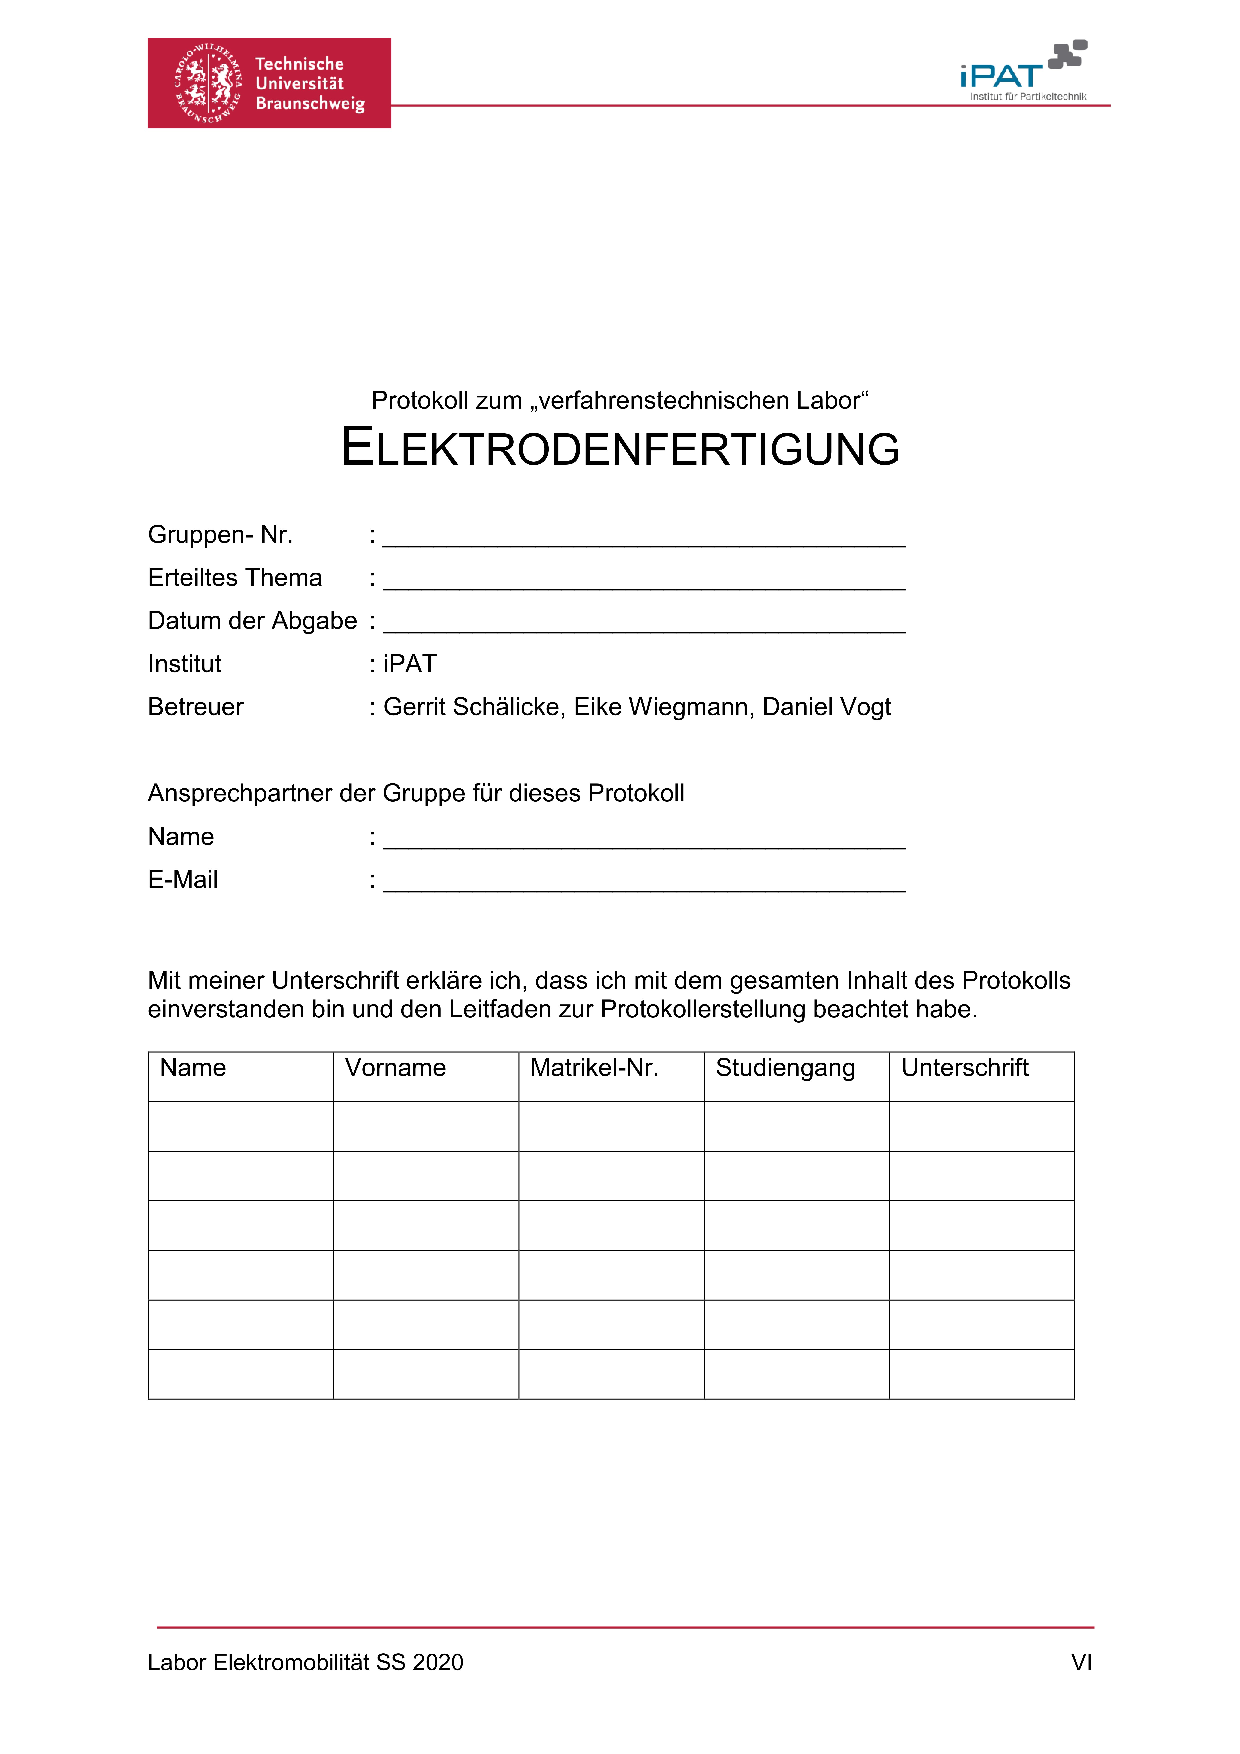
\includepdf[]{Titel_Blatt.pdf}
\tableofcontents
\newpage

\part{Abk\"urzungs- und Symbolverzeichnis}
\begin{table}[H]
    \centering
    \begin{tabular}{ccc}
        \midrule
        Abk\"urzung                   & Bedeutung                                   & Einheit      \\
        \toprule
        $RS$                          & Rakelspalt                                  & $\mu m$      \\
        $m_{Stl}$                     & Gewicht des Stanzlings                      & $\mu g$      \\
        \midrule
        \midrule
        Symbol                        & Bedeutung                                   & Einheit      \\
        \toprule
        $A_0$                         & Fl\"ache des Stanzlings                     & $cm^2$       \\
        $m_{i}$                       & Gewicht von $Probe_i$                       & $\mu g$      \\
        $\overline{m}$                & Mittelwert von $m_{i}$                      & $\mu g$      \\
        $\sigma_{m}$                  & Standardabweichung von $m_i$                & $\mu g$      \\
        $\rho_i$                      & Fl\"achengewicht von $Probe_i$              & $\mu g/cm^2$ \\
        $\overline{\rho}$             & Mittelwert von $\rho_i$                     & $\mu g/cm^2$ \\
        $\sigma_{\rho}$               & Standardabweichung von $\rho_i$             & $\mu g/cm^2$ \\
        $h_{Sch.,i}$                  & Schichtungsdicke von $Probe_i$              & $\mu m$      \\
        $\overline{h_{Sch.}}$         & Mittelwert von $h_{Sch.,i}$                 & $\mu m$      \\
        $\sigma_{h_{Sch.}}$           & Standardabweichung von $h_{Sch.,i}$         & $\mu m$      \\
        $h_{Besch.}$                  & Beschichtungsdicke von $Probe_i$            & $\mu m$      \\
        $\overline{h_{Besch.,i}}$     & Mittelwert von $h_{Besch.}$                 & $\mu m$      \\
        $\sigma_{h_{Besch.}}$         & Standardabweichung von $h_{Besch.}$         & $\mu m$      \\
        $h_{Sub.}$                    & Substratdicke                               & $\mu m$      \\
        $F_{min,i}$                   & Abrisskraft von $Probe_i$                   & $N$          \\
        $\overline{F_{min}}$          & Mittelwert von $F_{min}$                    & $N$          \\
        $\sigma_{F_{min}}$            & Standardabweichung von $F_{min}$            & $N$          \\
        $\sigma_{Zug,max,i}$          & Maximale Zugspannung von $Probe_i$          & $kPa$        \\
        $\overline{\sigma_{Zug,max}}$ & Mittelwert von $\sigma_{Zug,max,i}$         & $kPa$        \\
        $\sigma_{\sigma_{Zug,max}}$   & Standardabweichung von $\sigma_{Zug,max,i}$ & $kPa$        \\
        \midrule
    \end{tabular}

\end{table}

\newpage

\part{Einleitung}

\newpage

\part{Literaturrecherche}
\section{Analysemethoden in der
  Batterieverfahrenstechnik}

\subsection{XPS methode bei der Untersuchung des Kathodenmaterials LiCoO2}
In diesem Abschnitt werden die grundlegenden Eigenschaften des Kathodenmaterials
LiCoO2 beschrieben, welches mittels photoelektronenspekroskopie(XPS) hergestellt wurde.
\subsubsection{XPS Methode}
XPS basiert darauf, dass Elektronen aus gebundenen Zuständen in das Vakuum emittiert werden, wenn elektromagnetische Strahlung auf sie einwirkt. Aus der Energie der emittierten Elektronen kann dabei auf die Bindungszustände der Probe geschlossen werden.

Hier trifft Röntgenstrahlung der Energie hν auf eine Probe. Die Röntgenstrahlung wird dabei entweder durch die monochromatisierte Röntgenbremsstreuung von Aluminium, durch Helium-Gasentladung oder durch Synchrotronstrahlung erzeugt. Hierbei bietet das Synchrotron die Möglichkeit, die Energie frei zu variieren, während bei den anderen Methoden nur bestimmte, diskrete Anregungsenergien zur Verfügung stehen.Diese Strahlung emittiert ein Elektron aus der Probe, von wo es dann über einen Analysator energiedispersiv aufgelöst und an einem Channeltron detektiert wird. Aus der Energie der emittierten Elektronen kann anschließend die Bindungsenergie gewonnen werden.
\begin{figure}[H]
    \centering
    \begin{minipage}[t]{0.4\linewidth}
        \centering
        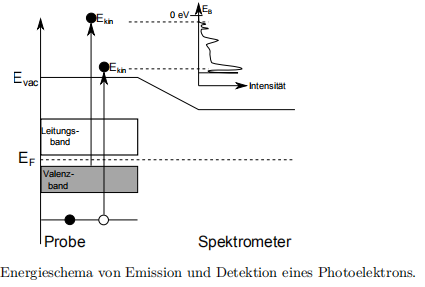
\includegraphics[width=\linewidth]{Diagramme/fig3_1_1.png}
        \caption{}
    \end{minipage}
    \begin{minipage}[t]{0.4\linewidth}
        \centering
        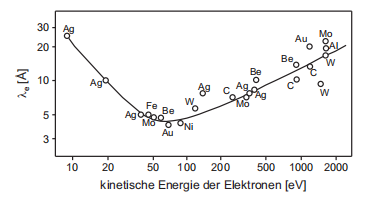
\includegraphics[width=\linewidth]{Diagramme/fig3_1_2.png}
        \caption{}
    \end{minipage}
\end{figure}

\subsubsection{Charakterisierung}
\begin{figure}[H]
    \centering
    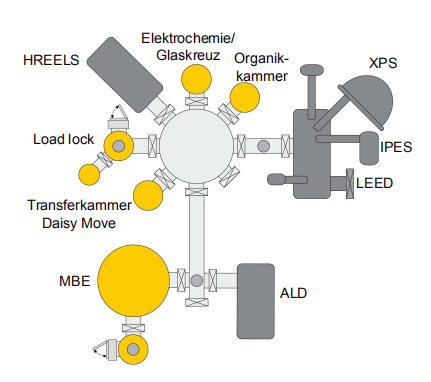
\includegraphics[width=.5\linewidth]{Diagramme/fig3_1_3.png}
    \caption{}
\end{figure}

Für beide XPS-Messsysteme wurde zur Kalibrierung eine metallische Silberprobe vermessen.

Die Messdaten wurden anschließend anhand der Verschiebung der Fermikante korrigiert.

Ein Fit mit derFermifunktion:
\begin{equation}
    A\dfrac{1}{exp({\dfrac{E-\Delta E}{k_B T})+1}}
\end{equation}

Für die Auswertung der gemessenen Spektren wurde der Untergrund in Form einer ShirleyFunktion [100] abgezogen. Für die Fits wurde eine Gauß-Lorentz-Funktion mit einem
konstanten Lorentz-Anteil von 30 Prozent (m = 0,3) verwendet, da dieses Verhältnis die
Messdaten am besten widerspiegelte:

\begin{equation}
    \dfrac{exp\left(-4\ln2(1-m)\dfrac{(x-E)^2}{w^2}\right)}{1+4m\dfrac{(x-E)^2}{w^2}}
\end{equation}

\subsubsection{Ergebniss}
In Abbildung3-4 ist eine Übersicht von XP-Spektren der gesputterten LiCoO2 Schichten
gezeigt, welche mit verschiedenen Anregungsenergien gemessen wurde: Hier werden für
Lithium, Cobalt, Sauerstoff und dem Valenzband Messungen mit einer Aluminium-Röntgenquelle sowie Messungen am Synchrotron gezeigt, wo die Proben oberflächensensitiv vermessen wurden.

Im Co2p Spektrum können zwei Hauptemissionen bei 779,8 eV und 794,7 eV beobachtet werden.Hier kann eine Komponente, die verglichen zur Hauptkomponente um 1,1 eV zu höheren Bindungsenergien verschoben ist, der Oxidationsstufe 2+ zugeordnet werden, eine Komponente mit Abstand von 6,0 eV der Oxidation 4+ und eine Komponente mit Abstand von 9,5 eV der Oxidationsstufe 3+ . Da die Cobaltspektren nur eine Komponente im Abstand von 9,5 eV zeigen, kommt im Wesentlichen nur die Oxidationsstufe 3+ vor, wie dies für stöchiometrisches LiCoO2 erwartet wird.

Im Sauerstoffspektrum gibt es zwei Komponenten bei 529,5 eV und 531,3 eV. Bei 531,3 eV ist in den Messungen am Synchrotron deutlich intensitätsstärker. Diese Komponente wird hauptsächlich auf Atome an der Oberfläche zurückgeführt, die eine unterschiedliche Ladung im Vergleich zu den Atomen im Festkörper besitzen.

\begin{figure}[H]
    \centering
    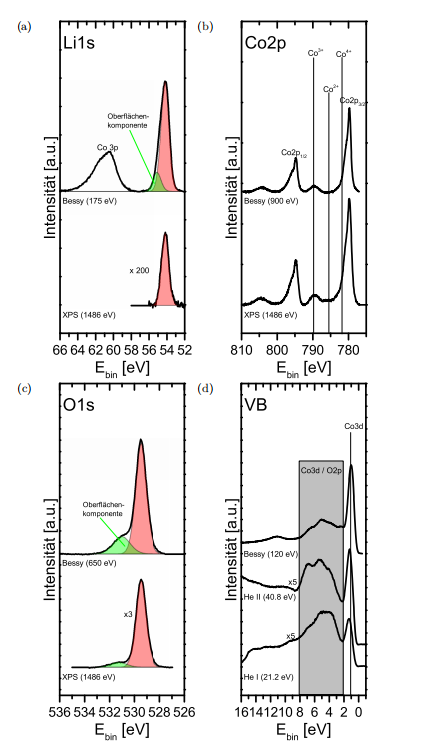
\includegraphics[width=.5\linewidth]{Diagramme/fig3_1_4.png}
    \caption{}
\end{figure}

Für das Valenzband von LiCoO2 wurden UPS-Messungen mit zwei Anregungsenergien(He I: 21,2 eV, He II: 40,8 eV) durchgeführt. Durch die unterschiedlichen Wirkungsquerschnitte bei den verschiedenen Anregungsenergien unterscheiden sich Form und Intensität dieser Spektren.

\begin{table}[H]
    \centering
    \caption{}
    \begin{tabular}{cccc}
        \midrule
                                & LiCoO$_2$             & Li$_2$O               & Li$_2$CO$_3$          \\
        \toprule
        Target                  & LiCoO$_2$             & Li$_2$O               & Li$_2$O               \\
        Kammer                  & Anode                 & Anode                 & Elektrolyt            \\
        Druck                   & 8$\cdot$10$^{-3}$mbar & 8$\cdot$10$^{-3}$mbar & 1$\cdot$10$^{-2}$mbar \\
        Fluss Argon             & 6sccm                 & 10sccm                & 0sccm                 \\
        Fluss Sauerstoff        & 6sccm                 & 0sccm                 & 0sccm                 \\
        Fluss Stickstoff        & 0sccm                 & 0sccm                 & 0sccm                 \\
        Fluss Kohlenstoffdioxid & 0sccm                 & 0sccm                 & 8sccm                 \\
        Temperatur              & 550\celsius           & 300\celsius           & 300\celsius           \\
        Abstand                 & 6,3cm                 & 6,3cm                 & 6,8cm                 \\
        Leistung                & 50W                   & 50W                   & 50W                   \\
        \midrule
    \end{tabular}
\end{table}

\subsection{Modellparametrierung durch EIS}
\subsubsection{EIS Methode}
Meist benutzen wir die elektrochemische Impedanyspektroskopie(EIS), um den Wechselstromwiderstand von der elekreochemischen Systeme zu bestimmen.

Da müssen wir zuerst einen ESB annehmen. Einfache ESB-Modelle zur Beschreibung des Innenwiderstands.Transportprozesse und Reaktionen in der Zelle sind verlustbehaftet und tragen zum Innenwiderstand  der Zelle bei

Es gibt drei Verlustpfade in Lithium-lonen Zellen:
\begin{enumerate}
    \item Ladungstransfer elektrochemische Reaktionen am Übergang Elektrode/Elektrolyt
    \item ohmsch ionische/elektronische Leitung in Elektrolyt und Elektroden
    \item Diffusion diffusiver Stofftransport von Reaktanden und Reaktionsprodukten
\end{enumerate}
\begin{figure}[H]
    \centering
    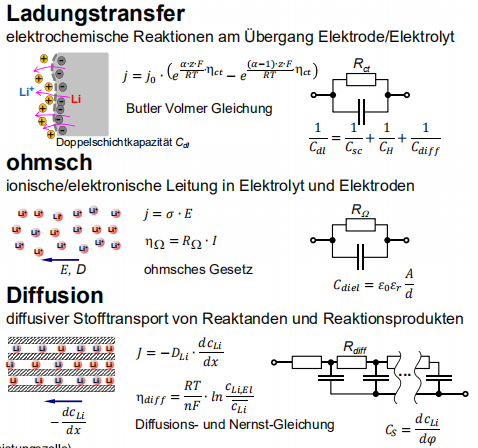
\includegraphics[width=.5\linewidth]{Diagramme/fig3_1_5.png}
    \caption{}
\end{figure}

\subsubsection{Einfaches Ersatzschaltbildmodell}
Für verschiedene Arten von Widerstand in der Batterie können wir die folgende Grundstruktur vereinfachen. Beispiel:

\begin{figure}[H]
    \centering
    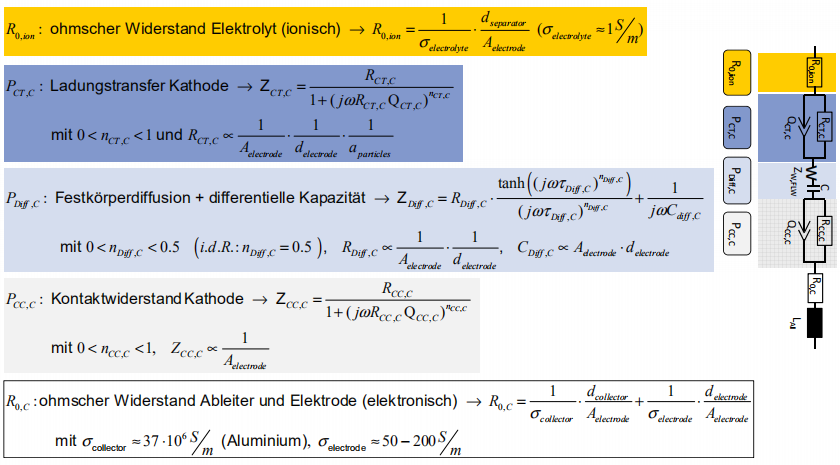
\includegraphics[width=.8\linewidth]{Diagramme/fig3_1_6.png}
    \caption{}
\end{figure}

Wir wissen, dass in verschiedenen Anwendungen Zellen mit unterschiedlichen Eigenschaften ausgewählt werden sollten.Dünne Elektroden kann besser n bei kurze Transportwege in den kleineren Elektroden angewandt werden.Dicke Elektroden haben größere Elektrodenvolumen : Batterievolumen Verhältnisse, welcher zur große Menge von Speicherung möglich führen.
Durch das REM können wir den Unterschied in der Mikrostruktur der Zellen in verschiedenen Anwendungen sehen.

\begin{figure}[H]
    \centering
    \begin{minipage}[t]{0.4\linewidth}
        \centering
        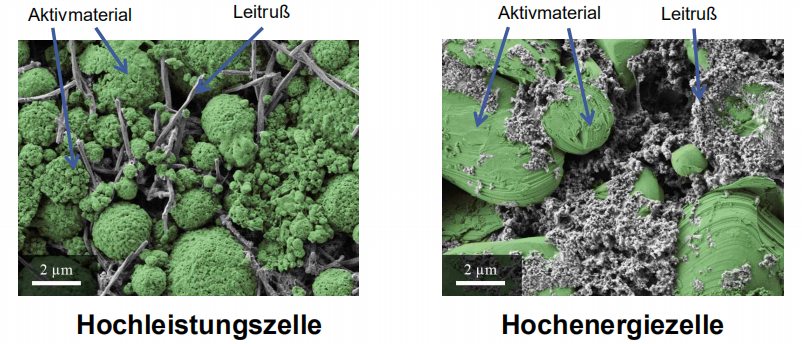
\includegraphics[width=\linewidth]{Diagramme/fig3_1_7.png}
    \end{minipage}
    \begin{minipage}[t]{0.4\linewidth}
        \centering
        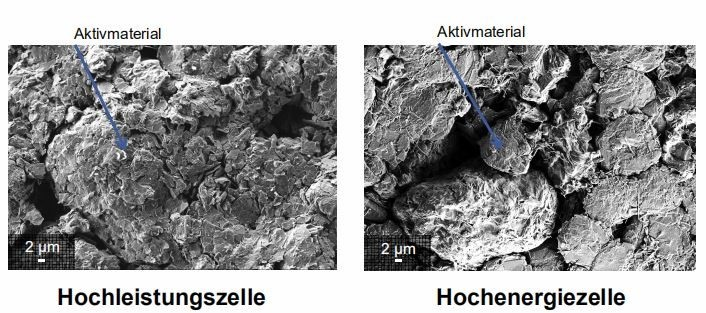
\includegraphics[width=\linewidth]{Diagramme/fig3_1_8.jpg}
    \end{minipage}
    \caption{}
\end{figure}

\subsubsection{Modellparametierung}
Messung des Potentialverlaufs $\varphi(r)=f(r,\sigma_{el},eff)$ und Maßder Fit Bewährte behördliche Leitfähigkeit und Kontaktwiderstand.Beim Untersuchung  benutzen wir einzelner Elektroden in ExperimentalzellenÖffnung \& Präparation kommerzieller Lithium-Ionen Batterien. Dann können wir einige Impedanzspektren von Anode bzw Kathode erstellen.

Beispiel:Ni0.6Mn0.2Co0.2 Kathode

\begin{figure}[H]
    \centering
    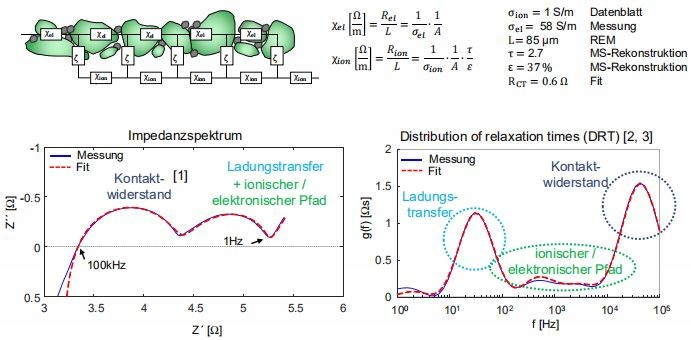
\includegraphics[width=.8\linewidth]{Diagramme/fig3_1_9.jpg}
    \caption{}
\end{figure}

\newpage
Durch Anpassen an den tatsächlichen Wert können wir das ESB der Elektrode durch die vorhergesagte Modelltopologie ableiten.

Quantifizierung der : Voxel insgesamt Mikrostrukturparameter
\begin{enumerate}
    \item  Vergleich von Strukturen
    \item  Einsatz in homogenisierten
    \item  Modellen
\end{enumerate}

\begin{figure}[H]
    \centering

    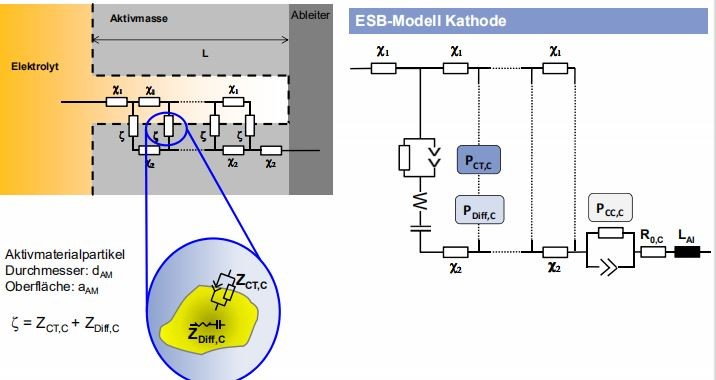
\includegraphics[width=.5\linewidth]{Diagramme/fig3_1_10.jpg}
    \caption{}
    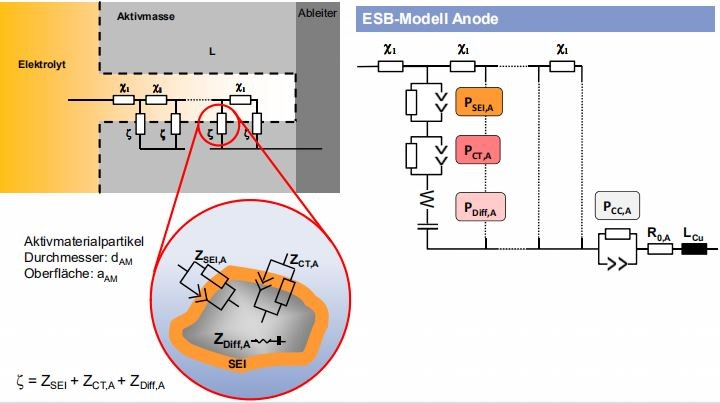
\includegraphics[width=.5\linewidth]{Diagramme/fig3_1_11.jpg}
    \caption{}
\end{figure}
\newpage

\section{Einfluss der Trocknung der l\"osungsmettelhaltigen Beschichtung}
In der Verfahrenstechnik für den Produktion der Batterie werden wesentliche 2 Teile umgefasst. Der erste Teil ist die Elektrodenproduktion, welche einschließlich Suspensionsherstellung, Beschichten/Trocken und Kalandrieren. Die zweiten Teile ist Zellproduktion. Es handelt sich um Konfektionierung, Herstellung Elektrodenpackage und Kontaktierung und Einhausung.
Die Trocknung spielt ein wichtiges Rollen in der Prozesskette, weil Schichtmorphologie und die Eigenschaften der Elektrode in der Batteriezelle durch Trocknungsprozess beeinflusst werden. Das Ziel der Trocknung ist zur Entfernung des Lösemittels bei vergleichsweise hohen Lösemittelanteilen in der Größenordnung von 40 – 60Gew.-\%, welche bezogen auf die Gesamtslurrymasse. [X1] In der Folgenden werden über den Einfluss der Beschichtungs- und Trochnungsprozessschritte beschreiben.
\subsection{Temperatur}
%Trocknungstemperatur ist einer der prim\"are Faktoren der Trocknungs prozess. Die Temperatur vom Substrat wird \"ublich kontrolliert zwischen 80\celsius\ und 130\celsius. H\"oher Trocknungstemperatur bedeutet h\"oher Trocknungsrate.
Nach der Suspensionsherstellung kommt es zu den Beschichtungs- und Trocknungsprozess. Während dieser Prozess wird die vorbreitet Suspension auf das Substrat aufgebracht. Um eine feine Schicht zu entstehen ist den Einfluss von Trocknungstemperatur zu beachten.
Abb.3.1 zeigt die Verteilung des Verhältnisses von elastisch zu total für unterschiedliche Trocknungstemperaturen. Eine beobachtete Erhöhung entsteht nach dem Mittelwert des Verhältnisses mit steigender Temperatur. Dies ist ein Ergebnis des Anstiegs bei der Entmischung des Bindemittels und sind der Ruß verantwortlich für die Elastizität in einer Elektrode. Daher ist die höhere Bindemittelkonzentration an der Elektrodenoberfläche auf die Erhöhung des elastischen Verhaltens zurückzuführen. [X1]
\begin{figure}[H]
    \centering
    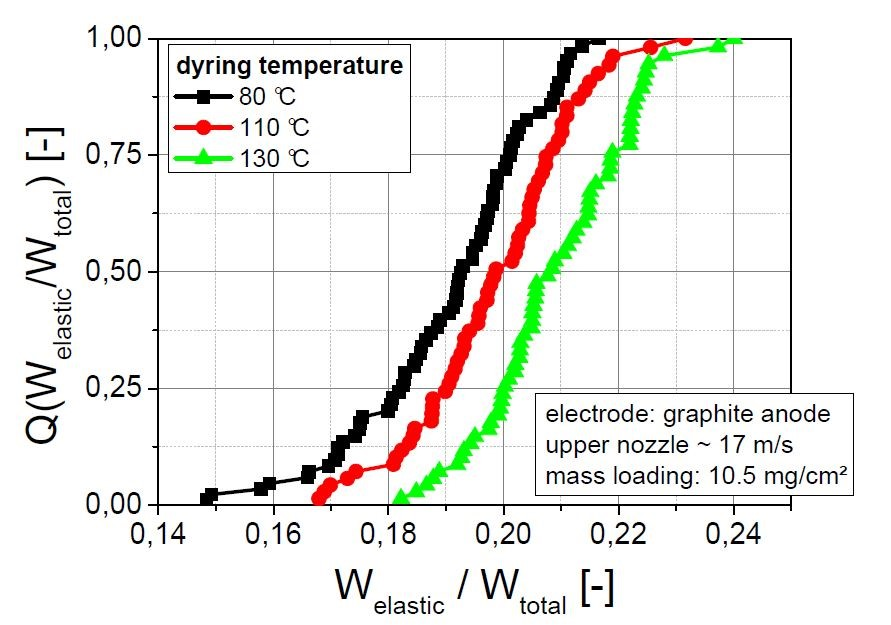
\includegraphics[width=.5\linewidth]{Diagramme/fig3_2_1.jpg}
    \caption{}
\end{figure}

Außerdem hat die Trockentemperatur ein Einfluss auf den Haftkraft der Beschichtung auf dem Substrat. Ein aus Experiment resultierende Abbildung mit unkalandrierten Elektrodenschichten zeigt, dass die Haftkraft mit steigender Temperatur abnimmt. Der Haftung zwischen den Partikeln und an der Substratfolie für die Leistung der Batteriezelle hat eine große Bedeutung. Delamination zwischen Aktivmaterialschicht und Stromleiter senkt die Leistungsfähigkeit der Batterie. Das ablösende einzelne Aktivmaterialpartikel bzw. größere Aktivmaterialdomänen kann einer deutlichen Absenkung der verfügbaren Zellkapazität zur Folger. [X2]
\begin{figure}[H]
    \centering
    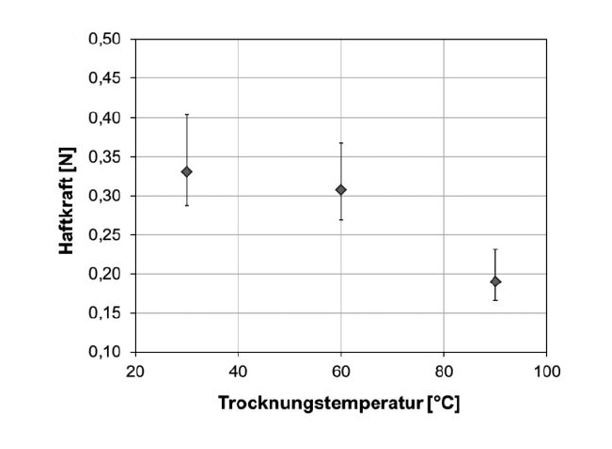
\includegraphics[width=.5\linewidth]{Diagramme/fig3_2_2.jpg}
    \caption{}
\end{figure}

\subsection{Massebeladung}
Weiterhin ist die Massebeladung einer Trocknungsprozess ein Einfluss an die Wiederstand an der Elektrode nachgewiesen. Abb. 3.4 zeigt, dass 5 zeigt, dass der elektrische Widerstand mit geringe Massebeladung fast kein Einfluss durch die steigende Temperatur hat, da die Gesamtmenge an Lösungsmittel gering ist und die Strukturimmobilisierung zu schnell ist, um eine signifikante Entmischung des Bindemittels zu bewirken. Aber die Elektrode mit hoher Massebeladung ist in Gegenseite. Einer höheren Antriebskraft für das Entmischen des Bindemittels und schließlich einem zunehmenden Widerstand ist wegen des Anstieges der Temperatur verantwortlich. [X1]
\begin{figure}[H]
    \centering
    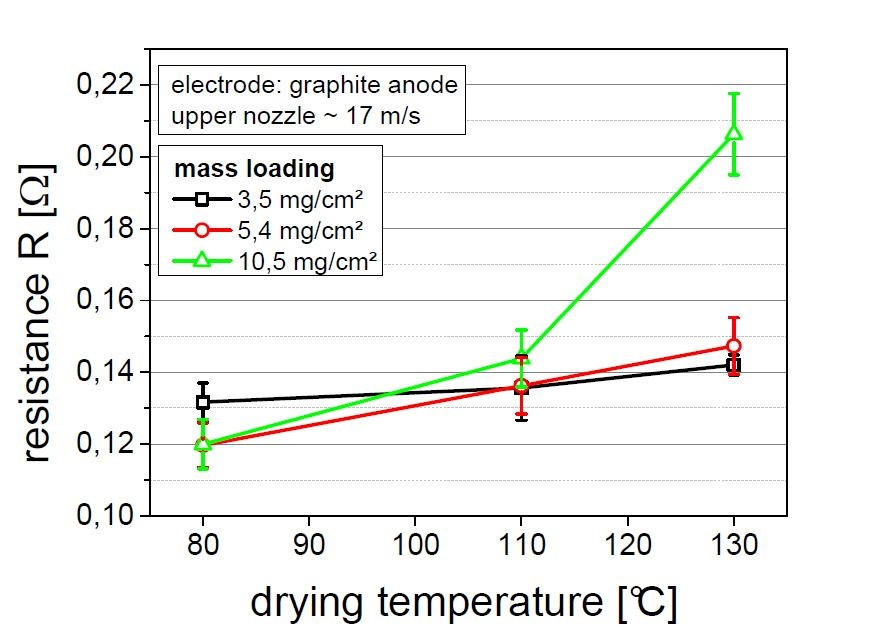
\includegraphics[width=.5\linewidth]{Diagramme/fig3_2_3.jpg}
    \caption{}
\end{figure}

\subsection{D\"usengeschwindigkeit / Luftstrom}
Düsen sind ein wichtiges Werkzeug in der Trocknungsprozess. Zu kontrollieren die Geschwindigkeit der Düsen hat eine große Bedeutung für die Trocknung. Es gibt 2 Arten der Düsen, nämlich die direkte (als hohe Geschwindigkeit) und diffuse (als niedrige Geschwindigkeit) Düsen. Führe Experiment hat zusammengefasst, dass die Geschwindigkeit auch Einfluss hat.
Abb 3.4 zeigt die Haftkraft über Geschwindigkeit mit verschiedene Massenbeladung. Es ist zu beobachten, dass einen Abfall entsteht, wenn Massenbelastung und Trocknungszeit hoch genug. In der Gegenseite werden geringere Massenbeladungen fast nicht von der höhere\linebreak Düsengeschwindigkeit beeinflusst, da die Trocknung zu schnell ist. Die Bindemittelgradienten werden durch Entmischen nicht hergestellt. [x1]
\begin{figure}[H]
    \centering
    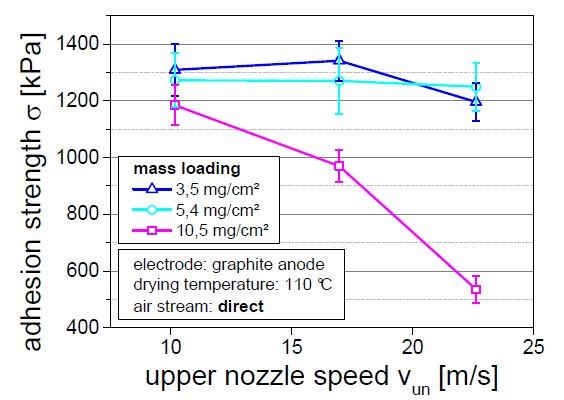
\includegraphics[width=.5\linewidth]{Diagramme/fig3_2_4.jpg}
    \caption{}
\end{figure}

\subsection{Trocknungsgrad}
Die Trocknungsrate hat sich auf die Kinetik der Strukturbildung und damit auf die Elektrodeneigenschaften ausgewirkt. Sie ist Basis auf dem Wärme- und Stofftransportbedingungen, welche eine Seite ein Einfluss von den Strömungsbedingungen der Trocknerluft haben und andere Seite von der Trocknungstemperatur über den Dampfdruck des Lösungsmittels. [X1]

%\subsubsection{Konvektion}Im Industrie werden nicht nur Aufheizung sondern auch erzwungene Konvektion angewendet. Das ist realisiert mit Zuluftventilatoren und D\"usen. Die Luftgeschwindigkeit kann durch Kontrolle \"uber Drehzahl von dem Ventilator reguliert werden. Durch Wahl zwischen verschiedene Orientierung von die D\"usen kann die Form vom Luftstrom variiert werden, n\"amlich zwischen direkt und Diffusion\cite{Westphal_2015}

%\subsubsection{Entsprechende Einfl\"usse auf die Elektrode}
%\paragraph{Einfluss auf die Struktur}
%\subparagraph{Entmischung}Gradient vom Binder durch ganze Folie\dots
%\paragraph{Eiflusse auf die Eigenschaften}
%\subparagraph{Adh\"asionskraft}
%Der Ad\"asionskraft von elektrode ist von Troknungskonditionen stark abh\"angig\cite{doi:10.1080/07373937.2015.1060497,Westphal_2015}.
%Die aus der Erh\"ohung der Trocknungsrate(engl. dryingrate) resultieredne Abnahme von Adh\"asionskraft von Elektrode werden beobachtet\cite{jaiser2016investigation}.
%\subparagraph{Elektrischer Volumenwiederstand}

%\subparagraph{Elastische und plastische Deformierungsenergie}
%\subparagraph{Elektrochemische Eigenschaften}Es wird boebachtet dass die aus Hohe Trocknungsrate(High Drying Rate)resultierenden Elektrode ein Verlust von Kapazit\"at zeigen\cite{jaiser2016investigation}...
\newpage



\part{Material und Methoden}
\section{Versuchsmaterial}

\newpage
\section{Versuchsschritte}

\newpage

\part{Auswertung der Laborversuche}
\section{Rohdaten}
\begin{table}[H]
    \centering
    \caption{Rohdaten}
    \begin{tabular}{ccccccc}
        \midrule
                                           &                & Probe 1                        & Probe 2      & Probe 3      & Probe 4      & Probe 5      \\
        \toprule
        \multirow{3}{*}{$m_{Stl}[mg]$}     & 50$\mu m\ RS$  & 15.2                           & 14.1         & 13.1         & 13.7         & 12.8         \\
                                           & 100$\mu m\ RS$ & 16.2                           & 16.1         & 16.1         & 15.6         & 16.1         \\
                                           & 150$\mu m\ RS$ & 19.0                           & 18.7         & 18.8         & 18.9         & 18.8         \\
        \toprule
        \multirow{3}{*}{$h_{Sch.}[\mu m]$} & 50$\mu m\ RS$  & 64                             & 58           & 52           & 53           & 46           \\
                                           & 100$\mu m\ RS$ & 74                             & 74           & 73           & 68           & 69           \\
                                           & 150$\mu m\ RS$ & 94                             & 88           & 94           & 92           & 91           \\
        \toprule
        \multirow{3}{*}{$F_{min}[N]$}      & 50$\mu m\ RS$  & -79.24736023                   & -74.66591644 & -70.60778809 & -65.46820068 & -65.46820068 \\
                                           & 100$\mu m\ RS$ & -50.39896393                   & -51.10709763 & -52.73678589 & -48.65811539 & -51.68948746 \\
                                           & 150$\mu m\ RS$ & -40.67362213                   & -41.86125565 & -30.47481155 & -52.01008987 & -48.30031204 \\
        \toprule
        $A_0$                              & $alle.\ RS$    & \multicolumn{5}{c}{1.13$cm^2$}                                                             \\
        \midrule
    \end{tabular}
\end{table}

\section{Datenveratbeitung}
%In diesem Arbeit wird nach notwendige mathematische Ableitung Matlab benutzt f\"ur Datenverarbeitung und Diagrammsgeneration. Die Quelltexten sind im Anhang anzushauen. Folgende sind die Ableitungsschritte.
In diesem Arbeit ist die Datenverarbeitung zweistufig. Ersten wird eine direkte numerische verbindung zwischen Rohndaten und gew\"unscht Werte mathematisch etabliert. Danach wird Matlab benutzt f\"ur Zahlenberechnung und Diagrammsgeneration. Folgende sind die Ableitungsschritte, und die Quelltexten sind im Anhang anzushauen.
%\newpage
\subsection{Flächengewicht}
Grunds\"atzlich haben wir f\"ur gleichen Rakelspalt:
\begin{center}
    \begin{equation}
        \left\{
        \begin{aligned}
            \rho_{i}                & =\dfrac{m_{i}}{A_{0}}-\dfrac{m_{Sub.}}{A_{0}},\quad i=1,2,\cdots,N.      \\
            \overline{\rho}         & =\dfrac{\sum\limits_{i=1}^{N}\rho_{i}}{N}                                \\
            %\sigma_{\rho}   & =\sqrt{\dfrac{\sum\limits_{i=1}^{N}(\rho_{i}-\overline{\rho})^{2}}{N}} \\
            \overline{m}            & =\dfrac{\sum\limits_{i=1}^{N}m_{i}}{N}                                   \\
            \dfrac{m_{Sub.}}{A_{0}} & =8.73\cdot10^3\dfrac{mg}{cm^3}\cdot10\cdot10^{-4}cm=8.73\dfrac{mg}{cm^2}
            %\sigma_{m}      & =\sqrt{\dfrac{\sum\limits_{i=1}^{N}(m_{i}-\overline{m})^{2}}{N}}       \\
            %N               & =5                                                                     \\
        \end{aligned}
        \right.
    \end{equation}
\end{center}

Nach Formableitung haben wir:
\begin{center}
    \begin{equation}
        \left\{
        \begin{aligned}
            \overline{\rho} & =\dfrac{\overline{m}}{A_0}-\dfrac{m_{Sub.}}{A_{0}} \\
            \sigma_{\rho}   & =\dfrac{\sigma_m}{A_0}                             \\
        \end{aligned}
        \right.
    \end{equation}
\end{center}
Mit geeignete Einheiten gewahlt haben wir:
\begin{center}
    \begin{equation}
        \left\{
        \begin{aligned}
            \overline{\rho}[mg/cm^2]  & =\dfrac{\overline{m}[\mu g]}{A_0[cm^2]}-8.73\dfrac{mg}{cm^2} \\
            \sigma_{\rho}[\mu g/cm^2] & =\dfrac{\sigma_m[\mu g]}{A_0[cm^2]}                          \\
        \end{aligned}
        \right.
    \end{equation}
\end{center}
%\newpage

\subsection{Beschichtungsdicke}
Grunds\"atzlich haben wir f\"ur gleichen Rakelspalt:
\begin{center}
    \begin{equation}
        \left\{
        \begin{aligned}
            h_{Besch.,i}          & =h_{Sch.,i}-h_{Sub.},\quad i=1,2,\cdots,N.    \\
            \overline{h_{Besch.}} & =\dfrac{\sum\limits_{i=1}^{N}h_{Besch.,i}}{N} \\
            %\sigma_{h_{Besch.}}   & =\sqrt{\dfrac{\sum\limits_{i=1}^{N}(h_{Besch.,i}-\overline{h_{Besch.}})^{2}}{N}} \\
            \overline{h_{Sch.}}   & =\dfrac{\sum\limits_{i=1}^{N}h_{Sch.,i}}{N}   \\
            %\sigma_{h_{Sch.}}     & =\sqrt{\dfrac{\sum\limits_{i=1}^{N}(h_{Sch.,i}-\overline{h_{Sch.}})^{2}}{N}}     \\
            %N                     & =5                                                                               \\
        \end{aligned}
        \right.
    \end{equation}
\end{center}

Nach Formableitung haben wir:
\begin{center}
    \begin{equation}
        \left\{
        \begin{aligned}
            \overline{h_{Besch.}} & =\overline{h_{Sch.}}-h_{Sub.} \\
            \sigma_{h_{Besch.}}   & =\sigma_{h_{Sch.}}            \\
        \end{aligned}
        \right.
    \end{equation}
\end{center}
Mit geeignete Einheiten gewahlt haben wir:
\begin{center}
    \begin{equation}
        \left\{
        \begin{aligned}
            \overline{h_{Besch.}}[\mu m] & =\overline{h_{Sch.}}[\mu m]-h_{Sub.}[\mu m] \\
            \sigma_{h_{Besch.}}[\mu m]   & =\sigma_{h_{Sch.}}[\mu m]                   \\
        \end{aligned}
        \right.
    \end{equation}
\end{center}
%\newpage

\subsection{Haftfestigkeit}
Die Haftfestigkeit bezieht sich auf die Fähigkeit eines Klebstoffs, an einer Oberfläche zu haften und zwei Oberflächen miteinander zu verbinden. Sie wird gemessen, indem die maximale Zugspannung bewertet wird, die zum Ablösen oder Lösen des Klebstoffs senkrecht zum Substrat erforderlich ist. Die Haftfestigkeit ist die maximal mögliche Zugspannung an der Grenzfläche. Es wird durch die Schichtdicke und die Retention des Lösemittels beeinflusst, wenn lösungsmittelhaltige Beschichtungen verwendet werden. In diesem Experiment ist der Einfluss des Rakelspalts auf Haftfestigkeit gesucht. Der Rakelspalt bewirkt unmittelbar die Beschichtungsdicke, was an früherer Stelle in diesem Bereicht schon eingegangen ist.

In diesem Teil ist die Haftfestigkeit der Elektroden mit Hilfe von Abrisskraft gemessen. Die gemessenen Zugkräfte $F_min$ bei verschiedenen Rakelspalten mit jeweils 5 Proben sind in folgenden Tabelle dargestellt.


\paragraph{}

Grunds\"atzlich haben wir f\"ur gleichen Rakelspalt:
\begin{center}
    \begin{equation}
        \left\{
        \begin{aligned}
            \sigma_{Zug,max,i}          & =-\dfrac{F_{min,i}}{A_0},\quad i=1,2,\cdots,N.      \\
            \overline{\sigma_{Zug,max}} & =\dfrac{\sum\limits_{i=1}^{N}\sigma_{Zug,max,i}}{N} \\
            %\sigma_{\sigma_{Zug,max}}   & =\sqrt{\dfrac{\sum\limits_{i=1}^{N}(\sigma_{Zug,max,i}-\overline{\sigma_{Zug,max}})^{2}}{N}} \\
            \overline{F_{min}}          & =\dfrac{\sum\limits_{i=1}^{N}F_{min,i}}{N}          \\
            %\sigma_{F_{min}}            & =\sqrt{\dfrac{\sum\limits_{i=1}^{N}(F_{min,i}-\overline{F_{min}})^{2}}{N}}                   \\
            %N                           & =5                                                                                           \\
        \end{aligned}
        \right.
    \end{equation}
\end{center}

Nach Formableitung haben wir:
\begin{center}
    \begin{equation}
        \left\{
        \begin{aligned}
            \overline{\sigma_{Zug,max}} & =\dfrac{\overline{F_{min}}}{A_0} \\
            \sigma_{\sigma_{Zug,max}}   & =\dfrac{\sigma_{F_{min}}}{A_0}   \\
        \end{aligned}
        \right.
    \end{equation}
\end{center}
Mit geeignete Einheiten gewahlt haben wir:
\begin{center}
    \begin{equation}
        \left\{
        \begin{aligned}
            \overline{\sigma_{Zug,max}}[kPa] & =\dfrac{\overline{F_{min}}[N]}{A_0[cm^2]/10} \\
            \sigma_{\sigma_{Zug,max}}[kPa]   & =\dfrac{\sigma_{F_{min}[N]}}{A_0[cm^2]/10}   \\
        \end{aligned}
        \right.
    \end{equation}
\end{center}
\newpage

\section{Ergebnisse und Diskussion}
\subsection{Flächengewicht}
\begin{figure}[H]
    \centering
    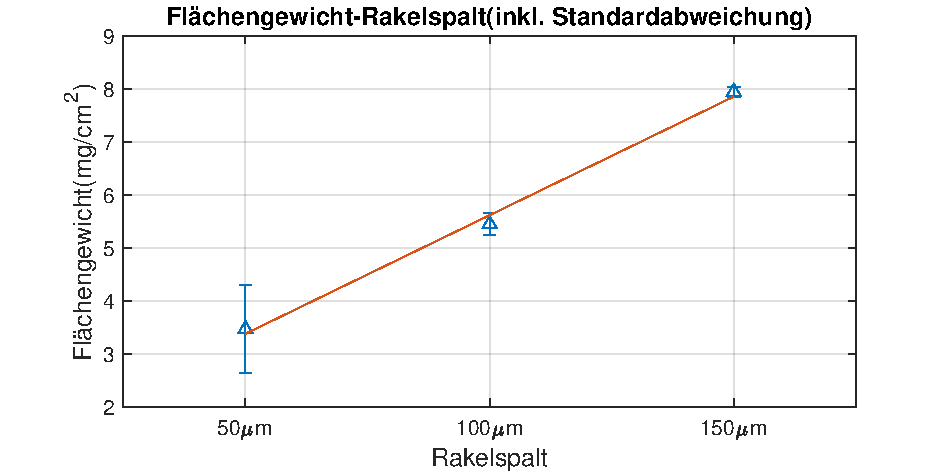
\includegraphics[]{Diagramme/Flaechengewicht.pdf}
\end{figure}

\begin{table}[H]
    \centering
    \caption{gew\"unschte Werte f\"ur Fl\"aschengewicht}
    \begin{tabular}{ccc}
        \midrule
        Rakelspalt[$\mu m$] & $\overline{\rho}[mg/cm^2]$ & $\sigma_{\rho}[\mu g/cm^2]$ \\
        \toprule
        50                  & 3.465                      & 0.833                       \\
        100                 & 5.447                      & 0.211                       \\
        150                 & 7.943                      & 0.101                       \\
        \midrule
    \end{tabular}
\end{table}

Eine positive Korrelation zwischen Rakelspalt und Fl\"aschengewicht kann hier beobachtet werden. Im gegebenen Raum von Rakelspalt darf diese Koorelation linear beschrieben werden, n\"amlich
\begin{center}
    \begin{equation}
        \left\{
        \begin{aligned}
            \rho[mg/cm^2] & =0.0448\cdot RS[\mu m]+1.1402 \\
            RS[\mu m]     & \in [50,150]                  \\
        \end{aligned}
        \right.
    \end{equation}
\end{center}
Der Schnittpunkt von diese Linie mit y-Achse liegt auf positive Halbachse, und zwar auf $(0,1.1402)$.Gleichzeitig ist die Standardabweichung bei 50$\mu m$ deutlich gr\"o\ss er als bei 100$\mu m$ und 150$\mu m$. Ein systematische Messfehler hat vielleicht passiert.

Wann wir diese Erscheinung nicht einfach als Fehler vernachl\"assigen,darf man spekulativ sagen, dass es auf eine Sedimentsschichte zur\"uckzuf\"uhren ist, welche bei niedriger Rakelspalt sichtlicher Effekt hat. F\"ur Nachpr\"ufung wird aber mehr Data ben\"otigt.
\subsection{Beschichtungsdicke}
\begin{figure}[H]
    \centering
    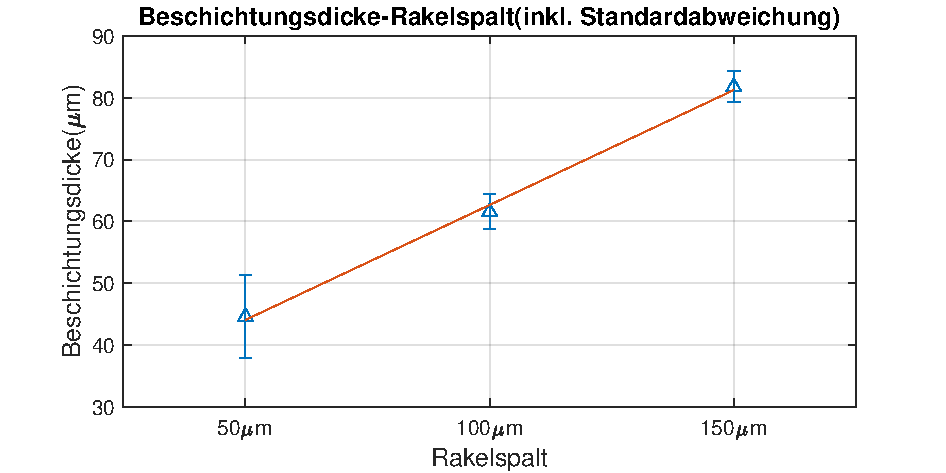
\includegraphics[]{Diagramme/Beschichtungsdicke.pdf}
\end{figure}

\begin{table}[H]
    \centering
    \caption{gew\"unschte Werte f\"ur Beschichtungsdicke}
    \begin{tabular}{ccc}
        \midrule
        Rakelspalt[$\mu m$] & $\overline{h_{Besch.}}[\mu m]$ & $\sigma_{h_{Besch.}}[\mu m]$ \\
        \toprule
        50                  & 44.6                           & 6.768                        \\
        100                 & 61.6                           & 2.881                        \\
        150                 & 81.8                           & 2.490                        \\
        \midrule
    \end{tabular}
\end{table}

Eine positive Korrelation zwischen Rakelspalt und Beschichtungsdicke kann hier beobachtet werden. Im gegebenen Raum von Rakelspalt darf diese Koorelation linear beschrieben werden, n\"amlich
\begin{center}
    \begin{equation}
        \left\{
        \begin{aligned}
            h_{Besch.}[\mu m] & =0.372\cdot RS[\mu m]+25.4667 \\
            RS[\mu m]         & \in [50,150]                  \\
        \end{aligned}
        \right.
    \end{equation}
\end{center}
Die Daten von Beschichtung haben \"ahnliche Charakteristiken wie die von
Fl\"achengewicht. Also der Schnittpunkt von diese Linie und y-Achse liegt auch auf positve Achse, und die Standardabweichung bei 50$\mu m$ ist auch deutlich gr\"o\ss er als bei 100$\mu m$ und 150$\mu m$. Nochmal spekulieren wir dass der Grund dahinter entweder eine systematische Messfehler oder Existenz von eine Sedimentsschichte ist.
\subsection{Haftfestigkeit}
\begin{figure}[H]
    \centering
    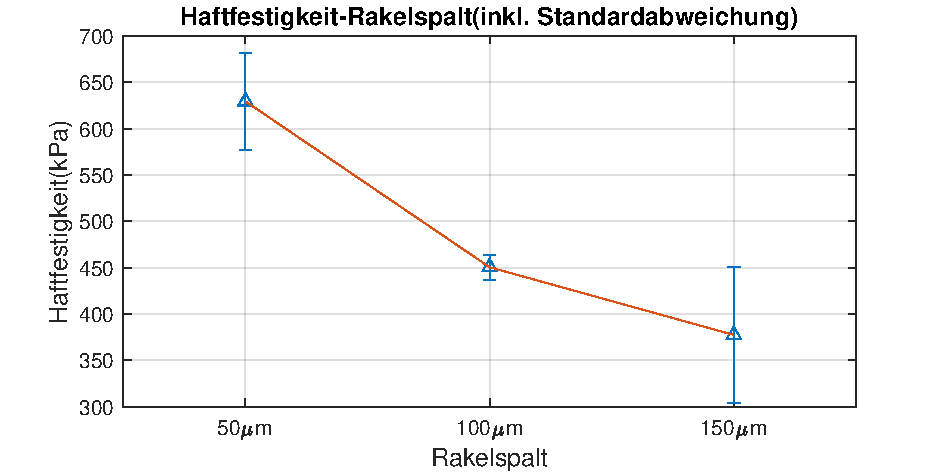
\includegraphics[]{Diagramme/Haftfestigkeit.pdf}
\end{figure}

\begin{table}[H]
    \centering
    \caption{gew\"unschte Werte f\"ur Haftfestigkeit}
    \begin{tabular}{ccc}
        \midrule
        Rakelspalt[$\mu m$] & $\overline{\sigma_{Zug,max}}[kPa]$ & $\sigma_{\sigma_{Zug,max}}[kPa]$ \\
        \toprule
        50                  & 629.58                             & 52.341                           \\
        100                 & 450.60                             & 13.505                           \\
        150                 & 377.56                             & 73.016                           \\
        \midrule
    \end{tabular}
\end{table}
Eine negative Korrelation zwischen Rakelspalt und maximale Zugspannung kann hier beobachtet werden. Im Experiment weist diese Beiziehung zwischen Haftfstigkeit und Rakelspalt eine nichtlineare Kennlinie auf.

Mit Betrachtung der Messdaten sind die Standardabweichung bei Rakelspalt von $150\mu m$ relativ groß. Das heißt, dass die Daten über eine relativ große Dispersität verfügen, die die Genauigkeit und Plausibilität des Experimentes beschädigen kann. Um die Abweichungen zu verkleinen, sollen mehr Stanzlinge ausgetanzt und analysiert. Eine der Gründe für diese große Abweichung ist dass mit steigende Rakelspalt die Schichtdicke auch zunimmt, damit kann der Stanzverfahren schwieriger werden und dabei größerer Impakt auftreten, der die Qualität des Stanzlings beeinflussen kann.

Das herauskommende Ergibnis entspricht dem erwarteten Ergebnis, das mit Hilfe von Literaturstellen begründet wird. Eine der möglichen Gründe für die Abnamme der Haftfestigkeit liegt daran, dass mit dickerer Beschichtung die Trocknung der Schicht unhomogen wird. Damit wird die innere Struktur und die Qualität der Beschictung beschädigt werden. Um die exakten Ursachen festzustellen, muss die Fehlerfläche weitergehend untersucht werden

\newpage

\part{Zusammenfassung}

\newpage

\clearpage
\renewcommand\refname{Literaturverzeichnis}
\bibliography{Literaturverzeichnis}
\newpage

\part{Anhang}
\section{Quelltexten}
\subsection{Teil Fl\"achengewicht}
\begin{lstlisting}
D_050=[15.2 14.1 13.1 13.7 12.8];
D_100=[16.2 16.1 16.1 15.6 16.1];
D_150=[19.0 18.7 18.8 18.9 18.8];
    
x = 50:50:150;
y = [mean(D_050) mean(D_100) mean(D_150)]/1.13;
err =[std(D_050) std(D_100) std(D_150)]/1.13;
    
errorbar(x,y,err,'--^')
grid on
title('Flaechengewicht-Rakelspalt(inkl. Standardabweichung)','FontSize',12)
xlabel('Rakelspalt','FontSize',12)
xlim([25 175])
xticks([50 100 150])
xticklabels({'50\mum','100\mum','150\mum'})
ylabel('Flaechengewicht(\mug/cm^2)','FontSize',12)

fig=gcf;
fig.PaperUnits='centimeters';
fig.PaperPosition=[0 0 16 10];
saveas(fig,'Flaechengewicht','svg')
saveas(fig,'Flaechengewicht','png')
\end{lstlisting}

\subsection{Teil Beschichtungsdicke}
\begin{lstlisting}
D_050=[64 58 52 53 46];
D_100=[74 74 73 68 69];
D_150=[94 88 94 92 91];
    
x = 50:50:150;
y = [mean(D_050)-10 mean(D_100)-10 mean(D_150)-10];
err =[std(D_050) std(D_100) std(D_150)];
    
errorbar(x,y,err,'--^')
grid on
title('Beschichtungsdicke-Rakelspalt(inkl. Standardabweichung)','FontSize',12)
xlabel('Rakelspalt','FontSize',12)
xlim([25 175])
xticks([50 100 150])
xticklabels({'50\mum','100\mum','150\mum'})
ylabel('Beschichtungsdicke(\mum)','FontSize',12)

fig=gcf;
fig.PaperUnits='centimeters';
fig.PaperPosition=[0 0 16 10];
saveas(fig,'Beschichtungsdicke','svg')
saveas(fig,'Beschichtungsdicke','png')
\end{lstlisting}

\subsection{Teil Haftfestigkeit}
\begin{lstlisting}
D_050=[79.24736023 74.66591644 70.60778809 65.46820068 65.72544861];
D_100=[50.39896393 51.10709763 52.73698589 48.65811539 51.68948746];
D_150=[40.67362213 41.86125565 30.47481155 52.01008987 48.30031204];

x = 50:50:150;
y = [mean(D_050) mean(D_100) mean(D_150)]/0.113;
err =[std(D_050) std(D_100) std(D_150)]/0.113;

errorbar(x,y,err,'--^')
grid on
title('Haftfestigkeit-Rakelspalt(inkl. Standardabweichung)','FontSize',12)
xlabel('Rakelspalt','FontSize',12)
xlim([25 175])
xticks([50 100 150])
xticklabels({'50\mum','100\mum','150\mum'})
ylabel('Haftfestigkeit(kPa)','FontSize',12)

fig=gcf;
fig.PaperUnits='centimeters';
fig.PaperPosition=[0 0 16 10];
saveas(fig,'Haftfestigkeit','svg')
saveas(fig,'Haftfestigkeit','png')
\end{lstlisting}
\end{document}